\documentclass[aspectratio=169]{beamer}
\usepackage[utf8]{inputenc}
%\usepackage[authordate,backend=biber,natbib]{biblatex-chicago}
%\usepackage{booktabs}
%\addbibresource{growthreferences.bib}

%\usepackage{utopia} %font utopia imported

\usetheme{Madrid}
\usecolortheme{beaver}

%------------------------------------------------------------
%This block of code defines the information to appear in the
%Title page
\title[Diamond (2016)] %optional
{The Determinants and Welfare Implications of US Workers Diverging Location Choices by Skill: 1980-2000}

\subtitle{Rebecca Diamond, \emph{American Economic Review}, 2016}

\author [Hauk] % (optional)
{William~R.~Hauk,~Jr.} %\inst{1} %\and J.~Doe\inst{2}} 

\institute[UofSC] % (optional)
{
  %\inst{1}%
  Darla Moore School of Business\\
  University of South Carolina
  %\and
  %\inst{2}%
  %Faculty of Chemistry\\
  %Very Famous University
}

\date[ECON 860, Fall 2021] % (optional)
{ECON 860 -- International Trade Theory\\Fall 2021}

\logo{
\includegraphics[height=1cm]{UofSC_Monogram_Stack_CMYK_G.jpg}}

%End of title page configuration block

%---------------------------------------------------------

\AtBeginSection[]
{
  \begin{frame}
    \frametitle{Table of Contents}
    \tableofcontents[currentsection,hideallsubsections]
  \end{frame}
}

%------------------------------------------------------------

\begin{document}

%The next statement creates the title page.
\frame{\titlepage}

%-------------------------------------------------------------

\section{Introduction}

%-------------------------------------------------------------

\begin{frame}{Introduction}

Paper looks at two stylized facts:
\begin{itemize}
    \item<1-> Dramatic increase in the wage gap between high school and college graduates in the U.S. between 1980-2000.
    \item<2-> Some metropolitan areas receiving an increasing share of college graduates during 1980-2000.
    \item<3-> Creates phenomenon of the ``Great Divergence”.
\end{itemize}
    
\end{frame}

%-------------------------------------------------------------

\begin{frame}{Welfare Implications}

\begin{itemize}
    \item<1-> If college graduates have higher nominal wages, but live in more expensive cities, are they necessarily better off?
    \item<2-> Welfare implications might depend on the reason why there is this skill sorting.
    \item<3-> Changes in relative demand for high and low skill workers were a big driver of migration patterns.
    \item<4-> However, once cities attracted more college graduates, they became more desirable and expensive places to live.
    \item<5-> High-wage workers were willing to pay for amenities of large cities, low-wage workers were not.
\end{itemize}
    
\end{frame}

%-------------------------------------------------------------

\begin{frame}{Welfare Implications}

\begin{itemize}
    \item<1-> Overall impact is to increase the gap in well-being between college graduates and high school graduates over and above what would be indicated simply from wage inequality.
    \item<2-> As an example, Diamond looks at differing fates of Detroit and Boston.
    \begin{itemize}
        \item<3-> Detroit loses auto manufacturing jobs, but also suffers from declining educational attainment.
        \item<4-> Boston has attracted high-skill workers and has increasing educational attainment.
    \end{itemize}
\end{itemize}

\end{frame}

%-------------------------------------------------------------

\begin{frame}{Methodology}

\begin{itemize}
    \item<1-> Paper uses a structural spatial equilibrium model of cities in the spirit of Rosen (1979) and Roback (1982), but allows for workers to have heterogeneous preferences for cities.
    \item<2-> Workers with different characteristics make different trade-offs.  The most important worker characteristic is skill level – operationalized by graduation from a four-year college.
    \item<3-> A city’s skill-mix will influence local amenity levels – paper looks at 15 amenities, which is combined into a single index using Principal Component Analysis (PCA).
\end{itemize}
    
\end{frame}

%-------------------------------------------------------------

\begin{frame}{Estimation}

\begin{itemize}
    \item<1-> Workers’ preferences for cities are estimated using a two-step estimator.
    \begin{enumerate}
        \item<2-> First step, MLE is used to identify how desirable a city is to each type of worker.
        \item<3-> Second step is to use a simultaneous-equation, non-linear GMM estimator to estimate local labor demand, housing supply, labor supply, and amenity supply to cities.
    \end{enumerate}
    \item<4-> Model is identified using local labor demand shocks from the local industry mix and their interactions with local housing supply elasticities. 
\end{itemize}
    
\end{frame}

%-------------------------------------------------------------

\begin{frame}{Punchline}

\begin{itemize}
    \item<1-> While both college and noncollege workers find higher wages, lower rents, and higher amenity levels desirable, high skill workers’ demand is relatively more sensitive to amenity levels and low skill workers’ demand is more sensitive to wages and rents.
    \item<2->   Welfare impacts from wage, rent, and endogenous amenity changes led to an increase in well-being equivalent to at least a 25\% increase in the college wage gap – which is larger than the actual increase in the college wage gap.
\end{itemize}
    
\end{frame}

%-------------------------------------------------------------

\begin{frame}{Is This a Trade Paper?}

\begin{itemize}
    \item<1-> JEL Codes classify this primarily as a Labor Economics paper.
    \item<2-> However, results are important for the way that we think about the welfare effects of trade.
    \item<3-> Papers we have looked at thus far assume that trade shocks cause a reallocation of labor to more ``efficient” uses.  But what if the adjustment costs are non-trivial?
    \item<4-> Diamond establishes facts that Autor, Dorn, and Hanson will elaborate on next week – jobs created by trade are not always in the same places as jobs lost by trade.  Adjustment costs may be substantial.
\end{itemize}
    
\end{frame}

%-------------------------------------------------------------

\section{Data}

%-------------------------------------------------------------

\begin{frame}{Census IPUMS Data}

\begin{itemize}
    \item<1-> Paper uses the 5 percent samples of the US census from the 1980, 1990, and 2000 Integrated Public Use Microdata Series (IPUMS) dataset.
    \item<2-> All analysis is restricted to 25-55 year-olds working at least 35 hours per week and 48 weeks per year.
    \item<3-> The geographical unit of analysis is the metropolitan statistical area (MSA) of residence.  Census includes 218 MSAs across all three decades of data.  Rural areas are not in an MSA, but rural areas within each state are grouped together as a single MSA.
\end{itemize}
    
\end{frame}

%-------------------------------------------------------------

\begin{frame}{Education and Amenities}

\begin{itemize}
    \item<1-> Workers divided into college degree or higher and no four-year college degree, as this seems to be the biggest dividing line between skilled and nonskilled workers according to Katz and Murphy (1992) and Goldin and Katz (2008).
    \item<2-> Key variable is the local skill mix (ratio of college workers to noncollege workers) of workers in an MSA.
    \item<3-> MSA amenities classified into six categories – retail, transportation, crime, environmental, schooling, and job quality.
    \item<4-> MSA data supplemented with measures of geographic constraints and land use regulations to measure differences in housing supply elasticities.
\end{itemize}
    
\end{frame}

%-------------------------------------------------------------

\section{Descriptive Statistics}

%-------------------------------------------------------------

\begin{frame}{Summary Statistics}

\begin{figure}
    \centering
    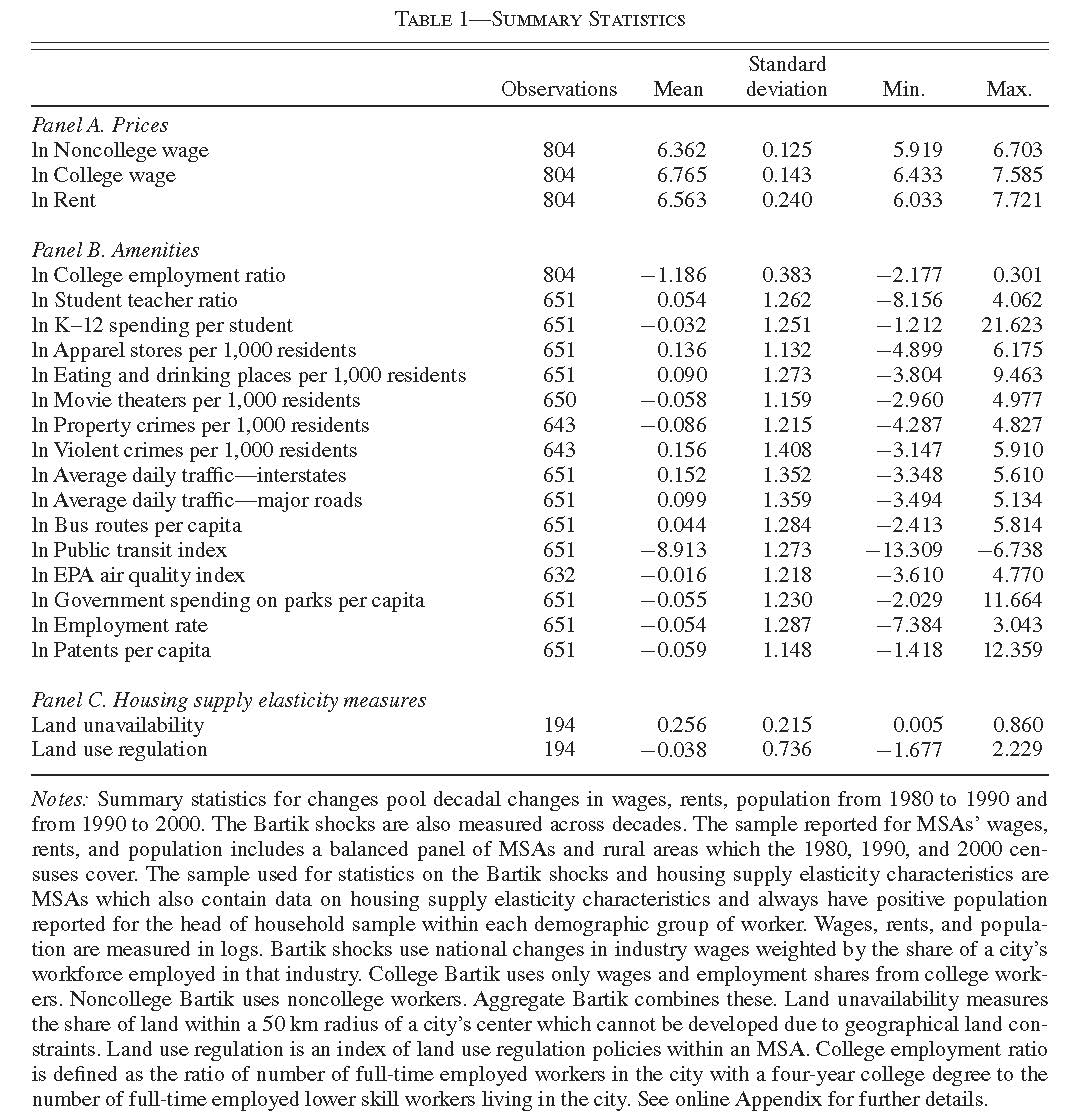
\includegraphics[scale=0.5]{DiamondTable1.jpg}
    \label{fig:Table1}
\end{figure}
    
\end{frame}

%-------------------------------------------------------------

\begin{frame}{Correlations}

\begin{figure}
    \centering
    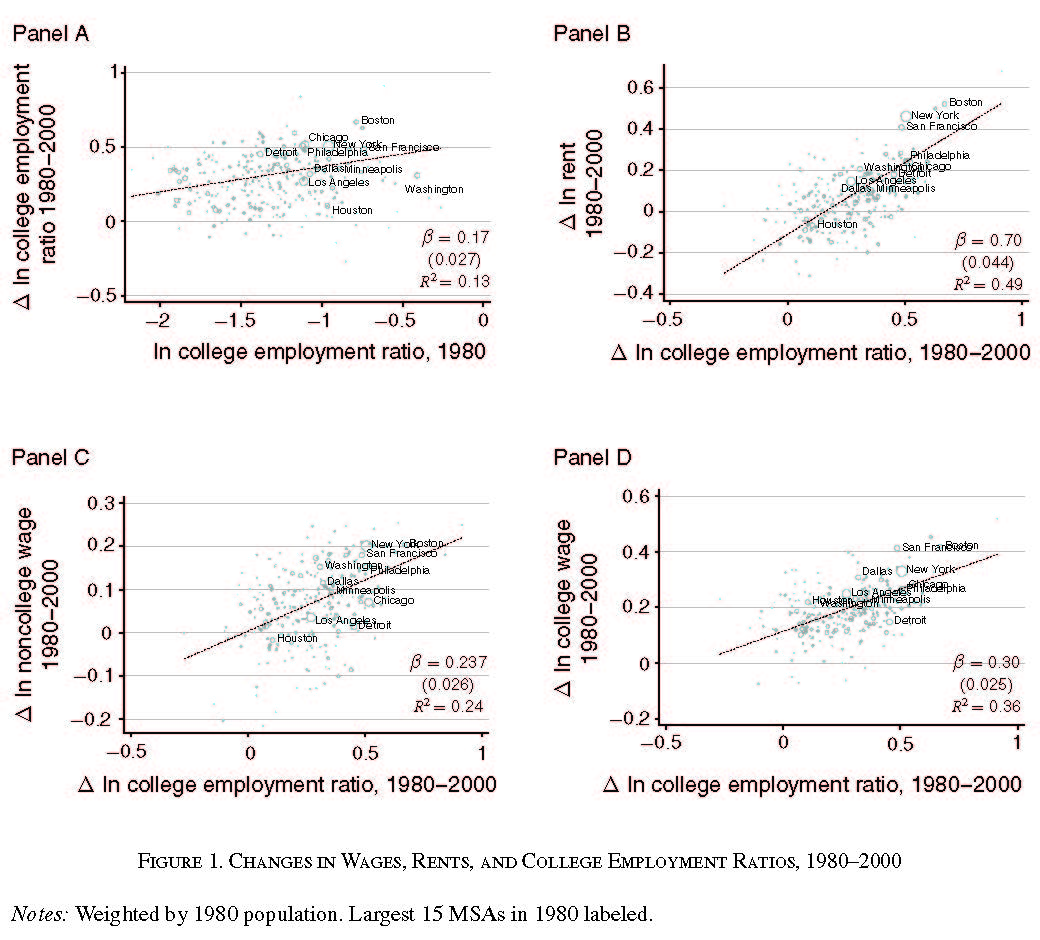
\includegraphics[scale=0.6]{DiamondFig1.jpg}
    \label{fig:Figure1}
\end{figure}
    
\end{frame}

%-------------------------------------------------------------

\begin{frame}{Correlations}

\begin{itemize}
    \item<1-> Panel A of Figure 1 shows that college employment ratio in 1980 is positively associated with growth in the college employment ratio from 1980-2000.  A 1\% increase in 1980 is associated with a 0.17\% larger increase from 1980-2000.
    \item<2-> Panel B of Figure 1 shows that an increase in the college employment ratio between 1980-2000 is positively associated with an increase in rents between 1980-2000.  A one percentage increase in college employment is associated with a 0.70\% increase in rents.
    \item<3-> Panel C of Figure 1 shows that an increase in the college employment ratio between 1980-2000 is positively associated with an increase in noncollege wages between 1980-2000.  A one percentage increase in college employment is associated with a 0.24\% increase in noncollege wages.
    \item<4-> Panel D of Figure 1 shows that an increase in the college employment ratio between 1980-2000 is positively associated with an increase in college wages between 1980-2000.  A one percentage in college employment is associated with a 0.30\% increase in college wages.
\end{itemize}
    
\end{frame}

%-------------------------------------------------------------

\begin{frame}{Wage Polarization}

The polarization of skill across cities coincided with a large nationwide increase in wage inequality.  Table 2 shows that the nationwide college/high school wage gap increased from 38\% in 1980 to 57\% in 2000.

\begin{figure}
    \centering
    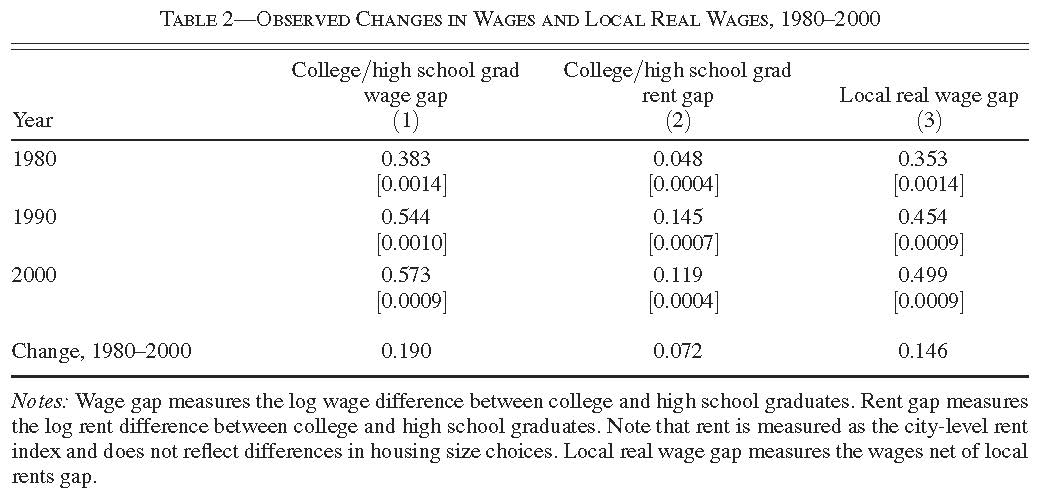
\includegraphics[scale=0.85]{DiamondTable2.jpg}
    \label{fig:Table2}
\end{figure}
    
\end{frame}

%-------------------------------------------------------------

\begin{frame}{Amenities Polarization}

Table 3 shows the relationships between changes in cities’ college employment ratios and their changes in a large set of local amenities.

\begin{figure}
    \centering
    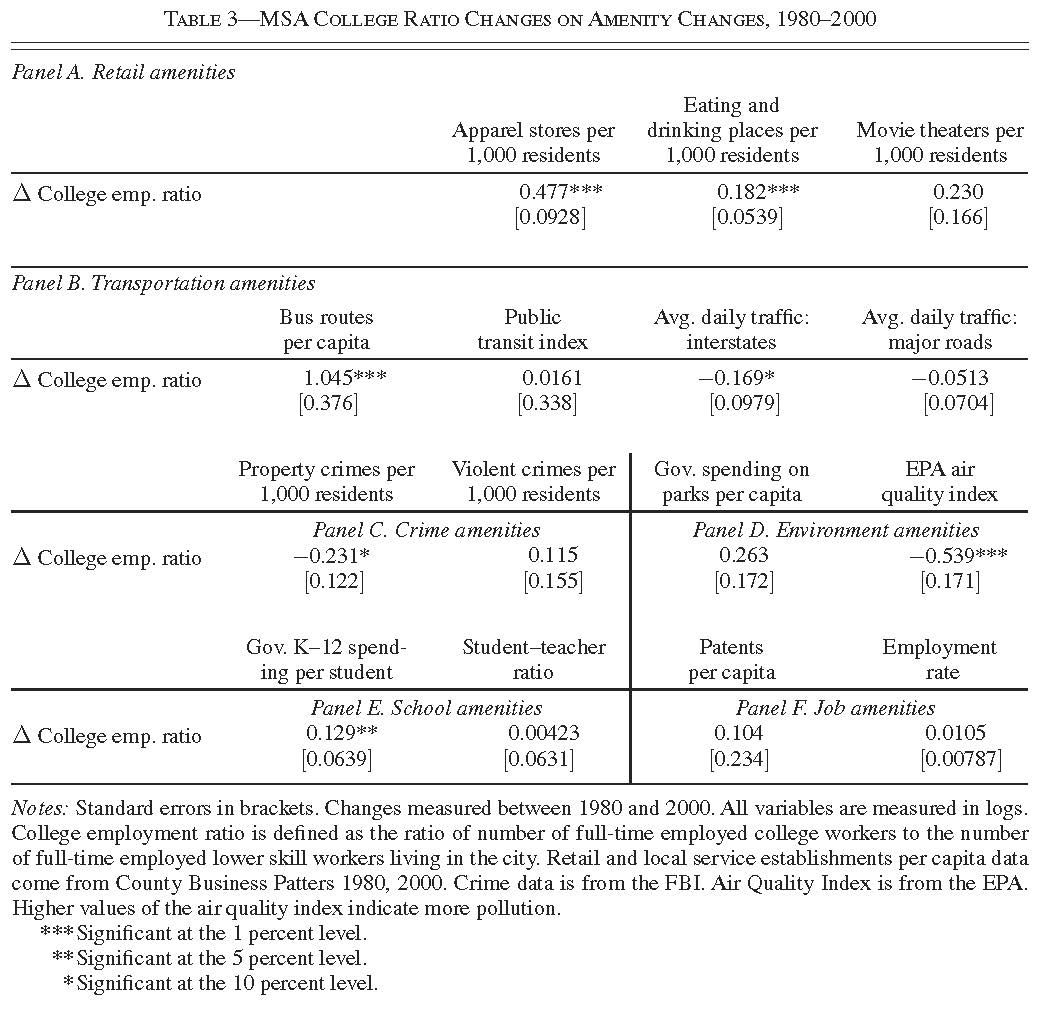
\includegraphics[scale=0.47]{DiamondTable3.jpg}
    \label{fig:Table3}
\end{figure}
    
\end{frame}

%-------------------------------------------------------------

\section{An Empirical Spatial Equilibrium Model of Cities}

%-------------------------------------------------------------

\begin{frame}{An Empirical Spatial Equilibrium Model of Cities}

\begin{itemize}
    \item<1-> In order to better understand how these observations affect welfare, one needs causal estimates of migration elasticities on these city characteristics.  Paper creates a structural model to estimate these elasticities.
    \item<2-> Structural model is similar to Rosen (1979) and Roback (1982), but allows more flexibility for heterogeneity in worker preferences and city housing supplies.
    \item<3-> Local worker productivity and amenities respond endogenously to the skill-mix of the city.
\end{itemize}
    
\end{frame}

%-------------------------------------------------------------

\subsection{Labor Demand}

%-------------------------------------------------------------

\begin{frame}{Labor Demand}

\begin{itemize}
    \item<1-> Each city $ j $ has many homogeneous firms $ d $ in year $ t $.
    \item<2-> These firms produce a homogeneous tradeable good using high skill labor $ H_{d,j,t} $, low skill labor $ L_{d,j,t} $, and capital $ K_{d,j,t} $ according to a Cobb-Douglas production function where high skill and low skill labor are substitutable:
    \begin{equation*}
        Y_{d,j,t} = N_{d,j,t}^{\alpha} K_{d,j,t}^{1 - \alpha}
    \end{equation*}
    where
    \begin{equation*}
        N_{d,j,t} = \left[ \theta_{j,t}^{L} L_{d,j,t}^{\rho} + \theta_{j,t}^{H} H_{d,j,t}^{\rho} \right]^{\frac{1}{\rho}}
    \end{equation*}
    and
    \begin{equation}
        \theta_{j,t}^{L} = f_{L}\left( H_{j,t}, L_{j,t} \right) \exp\left( e_{j,t}^L \right)
        \label{eq:lowskillproductivity}
    \end{equation}
    and
    \begin{equation}
        \theta_{j,t}^{H} = f_{H}\left( H_{j,t}, L_{j,t} \right) \exp\left( e_{j,t}^H \right)
        \label{eq:highskillproductivity}
    \end{equation}
\end{itemize}
    
\end{frame}

%-------------------------------------------------------------

\begin{frame}{Labor Productivity and Wages}

\begin{itemize}
    \item<1-> Equations (\ref{eq:lowskillproductivity}) and (\ref{eq:highskillproductivity}) show that labor productivity is determined by exogenous and endogenous factors.  Exogenous productivity shocks are given by the terms $ e_{j,t}^L $ and $ e_{j,t}^H $.
    \item<2-> While there is some evidence to indicate that the presence of more high skill workers leads to productivity spillovers for all workers, the functional form of the endogenous productivity functions $ f_L $ and $ f_H $ are agnostic for now.
    \item<3-> There are a large number of firms and no barriers to entry, so we can assume perfect competition and workers earn the value of their marginal product.  Capital is supplied elastically across all cities at price $ \kappa_t $. So:
    \begin{equation*}
        \begin{split}
            W_{j,t}^{H} &= \alpha N_{d,j,t}^{\alpha - \rho} K_{d,j,t}^{1 - \alpha} H_{d,j,t}^{\rho - 1} f_{H}\left( H_{j,t}, L_{j,t} \right) \exp\left( \varepsilon_{j,t}^{H} \right) \\
            W_{j,t}^{L} &= \alpha N_{d,j,t}^{\alpha - \rho} K_{d,j,t}^{1 - \alpha} L_{d,j,t}^{\rho - 1} f_{L}\left( H_{j,t}, L_{j,t} \right) \exp\left( \varepsilon_{j,t}^{L} \right) \\
            \kappa_{t} &= N_{d,j,t}^{\alpha} K_{d,j,t}^{-\alpha}\left( 1 - \alpha \right)
        \end{split}
    \end{equation*}
\end{itemize}
    
\end{frame}

%-------------------------------------------------------------

\begin{frame}{Aggregate Labor Demand}

Firm level labor demand translates directly into city-level aggregate labor demand as firms within a city all have an identical constant-returns-to-scale production technology:

\begin{equation*}
    \begin{split}
        w_{j,t}^{H} &= \log\left( W_{j,t}^H \right) = c_{t} + \left( 1 - \rho \right) \ log\left( N_{j,t} \right) + \left( \rho - 1 \right) \log \left( H_{j,t} \right) + \log\left( f_{H}\left( H_{j,t}, L_{j,t} \right) \right) + \varepsilon_{j,t}^{H} \\
        w_{j,t}^{L} &= \log\left( W_{j,t}^L \right) = c_{t} + \left( 1 - \rho \right) \ log\left( N_{j,t} \right) + \left( \rho - 1 \right) \log \left( L_{j,t} \right) + \log\left( f_{L}\left( H_{j,t}, L_{j,t} \right) \right) + \varepsilon_{j,t}^{L} \\
        N_{j,t} &= \left( \exp\left( \varepsilon_{j,t}^{L} \right) f_{L}\left( H_{j,t}, L_{j,t} \right) L_{j,t}^{\rho} + \exp\left( \varepsilon_{j,t}^{H} \right) f_{H}\left( H_{j,t}, L_{j,t} \right) H_{j,t}^{\rho} \right)^{\frac{1}{\rho}}
    \end{split}
\end{equation*}
where:
\begin{equation*}
    c_{t} = \log\left( \alpha \left( \frac{1 - \alpha}{\kappa_{t}} \right)^{\frac{1 - \alpha}{\alpha}} \right)
\end{equation*}
    
\end{frame}

%-------------------------------------------------------------

\begin{frame}{Aggregate Labor Demand}

\begin{itemize}
    \item<1-> Labor supply impacts wages through two channels: imperfect labor substitution of high and low skill workers within firms (governed by $ \rho $) and city wide productivity changes (governed by $ f_H $ and $ f_L $).
    \item<2-> Instead of imposing parametric restrictions, the labor demand functions can be rewritten as: \begin{equation*}
        \begin{split}
            w_{j,t}^{H} &= g_{H}\left( H_{j,t}, L_{j,t} \right) + \varepsilon_{j,t}^{H} \\
            w_{j,t}^{L} &= g_{L}\left( H_{j,t}, L_{j,t} \right) + \varepsilon_{j,t}^{L}
        \end{split}
    \end{equation*}
    \item<2-> We can approximate these functions using a log-linear specification:
    \begin{equation*}
        w_{j,t}^{H} = \gamma_{HH} \log{H_{j,t}} + \gamma_{HL} \log{L_{j,t}} + \varepsilon_{j,t}^{H}
    \end{equation*}
    and
    \begin{equation*}
        w_{j,t}^{L} = \gamma_{LH} \log{H_{j,t}} + \gamma_{LL} \log{L_{j,t}} + \varepsilon_{j,t}^{L}
    \end{equation*}
\end{itemize}
    
\end{frame}

%-------------------------------------------------------------

\subsection{Labor Supply to Cities}

%-------------------------------------------------------------

\begin{frame}{Labor Supply}

\begin{itemize}
    \item<1-> Each head-of-household worker $ i $ chooses to live in the city that offers him or her the most desirable bundle of wages, local good prices, and amenities, where wages are determined by the worker's education level.
    \item<2-> The worker consumes a local good $ M $, which has a local price $ R_{j,t} $, and a national good $ O $, which has a national price $ p_{t} $, and gains utility from the vector of amenities $ A_{j,t} $ in the city.
    \item<3-> The worker has Cobb-Douglas preferences for the local and national good, and the utility function looks like:
    \begin{equation*}
        \max_{M,O} \log\left( M^{\xi} \right) + \log\left( O^{1 - \xi} \right) + s_{i}\left( A_{j,t} \right)
    \end{equation*}
    subject to:
    \begin{equation*}
        P_{t} O + R_{j,t} M \le W_{j,t}^{edu}
    \end{equation*}
\end{itemize}
    
\end{frame}

%-------------------------------------------------------------

\begin{frame}{Worker's Utility}

\begin{itemize}
    \item<1-> The worker’s optimized utility function can be expressed as an indirect utility function
    \begin{equation*}
        V_{i,j,t} = \log\left( \frac{w_{j,t}^{edu}}{P_{t}} \right) - \xi \log\left( \frac{R_{j,t}}{P_{t}} \right) + s_{i} \left( A_{j,t} \right)
    \end{equation*}
    or
    \begin{equation}
        V_{i,j,t} = w_{j,t}^{edu} - \xi r_{j,t} + s_{i} \left( A_{j,t} \right)
        \label{eq:indirectutility1}
    \end{equation}
    \item<2-> The price index used in the denominator above, is the CPI-U index for all goods excluding shelter measured in year 2000 U.S. dollars.
    \item<3-> The workers’ optimized utility function also leads to his local good demand
    \begin{equation}
        HD_{i,j,t} = \frac{\xi w_{j,t}^{edu}}{R_{j,t}}
        \label{eq:localgooddemand}
    \end{equation}
\end{itemize}
    
\end{frame}

%-------------------------------------------------------------

\begin{frame}{Amenities and Labor Supply}

\begin{itemize}
    \item<1-> Some amenities are exogenous to the labor market mix of the city – define this as vector $ x_{j,t}^{A} $. Other amenities respond endogenously to the labor mix. Specifically, define $ a_{j,t} $ as the first principal comoponent of a bundle of amenities related to school quality, retail, crime, the environment, transportation, and the quality of the job market.
    \item<2-> The function $ s\left( A_{j,t} \right) $ maps the vector of city amenities to the worker's utility value for them:
    \begin{equation*}
        \begin{split}
            s\left( A_{j,t} \right) &= a_{j,t} \beta_{i}^{a} + x_{j,t}^{A} \beta_{i}^{x} + \beta_{i}^{st} x_{j}^{st} + \beta_{i}^{div} x_{j}^{div} + \sigma_{i} \varepsilon_{i,j,t} \\
            \beta_{i}^{x} &= \beta^{x} z_{i} \\
            \beta_{i}^{a} &= \beta^{a} z_{i} \\
            \beta_{i}^{st} &= st_{i} \beta^{st} z_{i} \\
            \beta_{i}^{div} &= div_{i} \beta^{div} z_{i} \\
            \sigma_{i} &= \beta^{\sigma} z_{i} \\
            \varepsilon_{i,j,t} &\sim \text{Type I Extreme Value}
        \end{split}
    \end{equation*}
\end{itemize}
    
\end{frame}

%-------------------------------------------------------------

\begin{frame}{Amenities and Labor Supply}

\begin{itemize}
    \item<1-> $ \beta_{i}^{st} $ and $ \beta_{i}^{div} $ measure a worker's value of living in his or her state of birth and census division of birth.
    \item<2-> Worker $ i $'s marginal utility of the different types of amenities are a function of a $ 3 \time 1 $ vector of demographic variables $ z_{i} $, which include dummy variables indicating if a worker is white, black, or an immigrant.
    \item<3-> $ x_{j}^{st} $ is a $ 50 \times 1 $ vector where each element $ k $ takes on a value of 1 if MSA $ j $ is partly located in state $ k $.  Similarly, $ x_{j}^{div} $ is a $ 9 \times 1 $ vector where element $ k $ takes on a value of 1 if MSA $ j $ is located in census division $ k $.
\end{itemize}
    
\end{frame}

%-------------------------------------------------------------

\begin{frame}{Utility Function Revisited}

\begin{itemize}
    \item<1-> $ \varepsilon_{i,j,t} $ is an idiosyncratic preference term for worker $ i $.  The indirect utility function (\ref{eq:indirectutility1}) is renormalized by dividing each worker’s utility by $ \beta^{\sigma} z_{i} $ so that the standard deviation of worker idiosyncratic preferences is normalized to 1.
    \item<2-> The indirect utility function for worker $ i $ in city $ j $ can now be written as:
    \begin{equation*}
        V_{i,j,t} = \left( w_{j,t}^{edu} - \xi r_{j,t} \right) \beta^{w} z_{i} + a_{j,t} \beta_{i}^{a} + x_{j,t} \beta_{i}^{x} + x_{j}^{st}\beta_{i}^{st} + x_{j}^{div} \beta_{i}^{div} + \varepsilon_{i,j,t}
    \end{equation*}
    \item<3-> Define $ \delta_{j,t}^{z} $ as the utility value of the components of city $ j $ that all workers of type $ z $ value identically:
    \begin{equation*}
        \delta_{j,t}^{z} = \left( w_{j,t}^{edu} - \xi r_{j,t} \right) \beta^{w} z_{i} + a_{j,t} \beta_{i}^{a} z_{i} + x_{j,t} \beta_{i}^{x} z_{i}
    \end{equation*}
    and rewriting the utility function in terms of $ \delta_{j,t}^{z} $, we have:
    \begin{equation*}
        V_{i,j,t} = \delta_{j,t}^{z} + x_{j}^{st}\beta_{i}^{st} z_{i} + x_{j}^{div} \beta_{i}^{div} z_{i} + \varepsilon_{i,j,t}
    \end{equation*}
\end{itemize}
    
\end{frame}

%-------------------------------------------------------------

\begin{frame}{Conditional Logit Model}

\begin{itemize}
    \item<1-> The total expected population of city j is simply the probability that each worker lives in the city, summed over all workers.  This can be rewritten as a conditional logit model for high skill workers:
    \begin{equation*}
        H_{j,t} = \sum_{i \in H_{t}} \frac{\exp\left( \delta_{j,t}^{z} + x_{j}^{st}\beta_{i}^{st} z_{i} + x_{j}^{div} \beta_{i}^{div} z_{i} \right)}{\sum_{k}^{J} \exp\left( \delta_{j,t}^{z} + x_{j}^{st}\beta_{i}^{st} z_{i} + x_{j}^{div} \beta_{i}^{div} z_{i} \right)}
    \end{equation*}
    and for low skill workers:
    \begin{equation*}
        L_{j,t} = \sum_{i \in L_{t}} \frac{\exp\left( \delta_{j,t}^{z} + x_{j}^{st}\beta_{i}^{st} z_{i} + x_{j}^{div} \beta_{i}^{div} z_{i} \right)}{\sum_{k}^{J} \exp\left( \delta_{j,t}^{z} + x_{j}^{st}\beta_{i}^{st} z_{i} + x_{j}^{div} \beta_{i}^{div} z_{i} \right)}
    \end{equation*}
    \item<2->Observed variables are the high and low skilled population, wages, rent, the amenity index, worker demographics, and workers’ states and census divisions of birth.  Exogenous amenities and idiosyncratic taste preferences are unobserved.  Estimated parameters are the workers’ preferences for wages, rent, and amenities ($ \beta $, $ \xi $).
\end{itemize}
    
\end{frame}

%-------------------------------------------------------------

\subsection{Housing Supply}

%-------------------------------------------------------------

\begin{frame}{Housing Supply}

\begin{itemize}
    \item<1-> Local prices $ R_{j,t} $, are set through equilibrium in the housing market.
    \item<2-> Developers are price takers and sell homogeneous houses at the marginal cost of production:
    \begin{equation*}
        P_{j,t}^{home} = MC\left( CC_{j,t}, LT_{j,t} \right)
    \end{equation*}
    where $ CC_{j,t} $ are local construction costs and $ LC_{j,t} $ are local land costs.
    \item<3-> In a steady-state real estate market equilibrium, there is no uncertainty and prices are equal to the discounted value of rents:
    \begin{equation*}
        R_{j,t} = \iota_{t} \times MC\left( CC_{j,t}, LT_{j,t} \right)
    \end{equation*}
    where $ \iota_{t} $ is the interest rate.
\end{itemize}
    
\end{frame}

%-------------------------------------------------------------

\begin{frame}{Housing Supply Equation}

\begin{itemize}
    \item<1->  The cost of land is a function of the aggregate demand for local goods given by equation (\ref{eq:localgooddemand}), which shows that local goods demand increases when wages rise or the price of local goods falls.  In-migration also affects housing demand.
    \item<2-> The log housing supply equation is parameterized as:
    \begin{equation*}
        \begin{split}
            r_{j,t} &= \log \left( R_{j,t} \right) = \log \left( \iota_{t} \right) + \log \left( CC_{j,t} \right) + \gamma_{j} \log \left( HD_{j,t} \right) \\
            \gamma_{j} &= \gamma + \gamma^{geo} \log\left( x_{j}^{geo} \right) + \gamma^{reg} \log\left( x_{j}^{reg} \right) \\
            HD_{j,t} &= L_{j,t} \frac{\xi w_{j,t}^{L}}{R_{j,t}} + H_{j,t} \frac{\xi w_{j,t}^{H}}{R_{j,t}}
        \end{split}
    \end{equation*}
    \item<3-> We can observe housing rent, land availability, land-use regulation, and local good demand.  Construction costs and the interest rate are unobserved.  Parameters to be estimated are housing supply elasticities ($ \gamma $) and the local good expenditure share ($ \xi $).
\end{itemize}
    
\end{frame}

%-------------------------------------------------------------

\subsection{Amenity Supply}

%-------------------------------------------------------------

\begin{frame}{Amenity Supply}

\begin{itemize}
    \item<1-> Some amenities supplied in a city are due to exogenous factors outside the model, these amenities are represented by the vector $ x_{j,t}^{A} $.
    \item<2-> Some amenities respond endogenously to the types of residents who live in the city.  The bundle of observable amenities will be represented by $ a_{j,t} $ (which is the first principal component of a large vector of amenities).
\end{itemize}
    
\end{frame}

%-------------------------------------------------------------

\begin{frame}{Amenity Supply Equation}

\begin{itemize}
    \item<1-> The level of the endogenous amenity index is determined by the high skill employment ratio $ \frac{H_{j,t}}{L_{j,t}} $.
    \begin{equation*}
        a_{j,t} = \gamma^{a} \log \left( \frac{H_{j,t}}{L_{j,t}} \right) + \varepsilon_{j,t}^{a}
    \end{equation*}
    \item<2-> We can observe the MSAs’ state, census division, and endogenous amenities, and the college employment ratio.  Exogenous amenities and the exogenous component of the amenity index are unobserved.  The elasticity of amenity supply ($ \gamma^{a} $) is estimated.
\end{itemize}
    
\end{frame}

%-------------------------------------------------------------

\subsection{Equilibrium}

%-------------------------------------------------------------

\begin{frame}{Equilibrium \#1}

Equilibrium in the model is defined by a menu of wages, rents, and amenity levels with populations such that:

\begin{itemize}
    \item<1-> The high skill labor demand equals high skill labor supply:
    \begin{equation}
        \begin{split}
            H_{j,t}^{*} &= \sum_{i \in H_{t}} \frac{\exp\left( \delta_{j,t}^{z} + x_{j}^{st}\beta_{i}^{st} z_{i} + x_{j}^{div} \beta_{i}^{div} z_{i} \right)}{\sum_{k}^{J} \exp\left( \delta_{j,t}^{z} + x_{j}^{st}\beta_{i}^{st} z_{i} + x_{j}^{div} \beta_{i}^{div} z_{i} \right)} \\
            w_{j,t}^{H^*} &= \gamma_{HH} \log \left( H_{j,t}^{*} \right) + \gamma_{HL} \log \left( L_{j,t}^{*} \right) + \varepsilon_{j,t}^{H} 
            \label{eq:wagehigh}
        \end{split}
    \end{equation}
    \item<2-> The low skill labor demand equals low skill labor supply:
    \begin{equation}
        \begin{split}
            L_{j,t}^{*} &= \sum_{i \in L_{t}} \frac{\exp\left( \delta_{j,t}^{z} + x_{j}^{st}\beta_{i}^{st} z_{i} + x_{j}^{div} \beta_{i}^{div} z_{i} \right)}{\sum_{k}^{J} \exp\left( \delta_{j,t}^{z} + x_{j}^{st}\beta_{i}^{st} z_{i} + x_{j}^{div} \beta_{i}^{div} z_{i} \right)} \\
            w_{j,t}^{L^*} &= \gamma_{LH} \log \left( H_{j,t}^{*} \right) + \gamma_{LL} \log \left( L_{j,t}^{*} \right) + \varepsilon_{j,t}^{L} 
            \label{eq:wagelow}
        \end{split}
    \end{equation}
\end{itemize}
    
\end{frame}

%-------------------------------------------------------------

\begin{frame}{Equilibrium \#2}

\begin{itemize}
    \item<1-> Housing demand equals housing supply:
    \begin{equation*}
        \begin{split}
            r_{j,t}^{*} &= \log\left( \iota_t \right) + \log\left( CC_{j,t} \right) + \gamma_{j} \log\left( HD_{j,t}^{*} \right) \\
            HD_{j,t}^{*} &= L_{j,t}^{*} \frac{\xi \exp\left( w_{j,t}^{L^*} \right)}{\exp\left( r_{j,t}^{*} \right)} + H_{j,t}^{*} \frac{\xi \exp\left( w_{j,t}^{H^*} \right)}{\exp\left( r_{j,t}^{*} \right)}
        \end{split}
    \end{equation*}
    \item<2-> Endogenous amenities demand equals endogenous amenities supply:
    \begin{equation*}
        \begin{split}
            a_{j,t}^{*} &= \gamma^{a} \log\left( \frac{H_{j,t}^{*}}{L_{j,t}^{*}} \right) + \varepsilon_{j,t}^{a} \\
            \delta_{j,t}^{z} &= \left( w_{j,t}^{edu^*} - \xi r_{j,t}^{*} \right) \beta^{w} z + a_{j,t}^{*} \beta_{i}^{a} z + x_{j,t}^{a} \beta_{i}^{x} z, \forall z
        \end{split}
    \end{equation*}
\end{itemize}

\end{frame}

%-------------------------------------------------------------

\section{Estimation}

\subsection{Endogenous Amenity Index}

%-------------------------------------------------------------

\begin{frame}{Estimating the Endogenous Amenity Index}

\begin{itemize}
    \item<1-> Data is collected on 15 different amenities, which are grouped into 6 categories: retail, transportation, crime, environment, school quality, and job quality (beyond wages).  Amenities are combined into a single index $ a_{j,t} $ using a principal components analysis.
    \item<2->  In order to avoid overweighting one category, analysis first creates a PCA index within each category, and then creates a PCA with each category’s index.  Table 4 shows the various weightings.
\end{itemize}
    
\end{frame}

%-------------------------------------------------------------

\begin{frame}{Table 4}

\begin{figure}
    \centering
    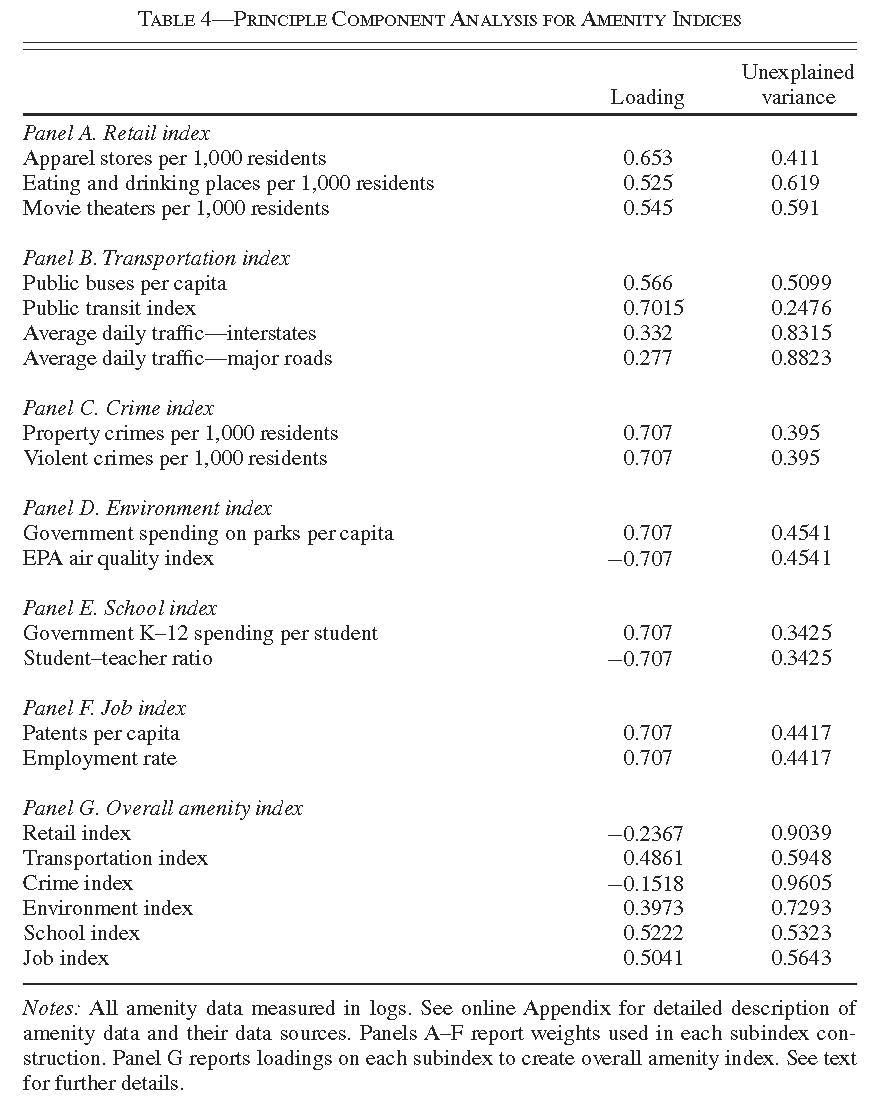
\includegraphics[scale=0.5]{DiamondTable4.jpg}
    \label{fig:Table4}
\end{figure}
    
\end{frame}

%-------------------------------------------------------------

\subsection{Bartik Labor Demand Shocks}

%-------------------------------------------------------------

\begin{frame}{Bartik Labor Demand Shocks}

\begin{itemize}
    \item<1->  Key to identifying model parameters is estimating how cities’ economic outcomes respond to exogenous shocks in local firm productivities based on Bartik (1991).
    \item<2-> The Bartik shocks for high and low skill workers are:
    \begin{equation*}
        \begin{split}
            \Delta B_{j,t}^{H} &= \sum_{ind}\left( w_{ind, -j,t}^{H} - w_{ind, -j,1980}^{H} \right) \frac{H_{ind,j,1980}}{H_{j,1980}} \\
            \Delta B_{j,t}^{L} &= \sum_{ind}\left( w_{ind, -j,t}^{L} - w_{ind, -j,1980}^{L} \right) \frac{L_{ind,j,1980}}{L_{j,1980}}
        \end{split}
    \end{equation*}
    where $ w_{ind, -j,t}^{H} $ and $ w_{ind, -j,t}^{L} $ are the average log wages of high and low skill workers in industry $ ind $ in cities other than $ j $ in year $ t $.
\end{itemize}
    
\end{frame}

%-------------------------------------------------------------

\begin{frame}{Bartik Shocks and Labor Demand}

Bartik labor demand shocks are a component of a city’s exogenous productivity changes over time.  The productivity changes from equations (\ref{eq:wagehigh}) and (\ref{eq:wagelow}) can be written as:
\begin{equation}
    \Delta \varepsilon_{j,t}^{H} = \gamma_{BHH} \Delta B_{j,t}^{H} + \gamma_{BHL} \Delta B_{j,t}^{L} + \Delta \tilde{\varepsilon}_{j,t}^{H}
    \label{eq:Bartikshockhigh2}
\end{equation}
\begin{equation}
    \Delta \varepsilon_{j,t}^{L} = \gamma_{BLH} \Delta B_{j,t}^{H} + \gamma_{BLL} \Delta B_{j,t}^{L} + \Delta \tilde{\varepsilon}_{j,t}^{L}
    \label{eq:Bartikshocklow2}
\end{equation}
    
\end{frame}

%-------------------------------------------------------------

\subsection{Labor Demand}

%-------------------------------------------------------------

\begin{frame}{Labor Demand}

\begin{itemize}
    \item<1-> Using equations (\ref{eq:wagehigh}) and (\ref{eq:wagelow}) and differencing cities’ wages relative to their 1980 levels gives us:
    \begin{equation}
        \Delta w_{j,t}^{H} = \gamma_{HH} \Delta H_{j,t} + \gamma_{HL} \Delta L_{j,t} + \Delta \varepsilon_{j,t}^{H}
        \label{eq:wagechangehigh}
    \end{equation}
    \begin{equation}
        \Delta w_{j,t}^{L} = \gamma_{LH} \Delta H_{j,t} + \gamma_{LL} \Delta L_{j,t} + \Delta \varepsilon_{j,t}^{L}
        \label{eq:wagechangelow}
    \end{equation}
    \item<2-> Plugging the Bartik shock equations (\ref{eq:Bartikshockhigh2}) and (\ref{eq:Bartikshocklow2}) into the wage change equations (\ref{eq:wagechangehigh}) and (\ref{eq:wagechangelow}) gives us:
    \begin{equation*}
        \Delta w_{j,t}^{H} = \gamma_{HH} \Delta H_{j,t} + \gamma_{HL} \Delta L_{j,t} + \gamma_{BHH} \Delta B_{j,t}^{H} + \gamma_{BHL} \Delta B_{j,t}^{L}+ \Delta \tilde{\varepsilon}_{j,t}^{H}
    \end{equation*}
    \begin{equation*}
        \Delta w_{j,t}^{L} = \gamma_{LH} \Delta H_{j,t} + \gamma_{LL} \Delta L_{j,t} + \gamma_{BLH} \Delta B_{j,t}^{H} + \gamma_{BLL} \Delta B_{j,t}^{L}+ \Delta \tilde{\varepsilon}_{j,t}^{L}
    \end{equation*}
\end{itemize}

\end{frame}

%-------------------------------------------------------------

\begin{frame}{Bartik Shocks and Exclusion Restrictions}

\begin{itemize}
    \item<1->  The Bartik shocks provide plausibly exogenous labor demand shifters.  The labor demand elasticities will be identified through variations in the labor supply that come through housing supply.
    \item<2-> In order for housing supply to help to identify labor market equilibrium, we need to make the following exclusion restrictions:
    \begin{equation*}
        \begin{split}
            E\left[ \Delta \tilde{\varepsilon}_{j,t}^{H} , \Delta Z_{j,t} \right] &= 0 \\
            E\left[ \Delta \tilde{\varepsilon}_{j,t}^{L} , \Delta Z_{j,t} \right] &= 0
        \end{split}
    \end{equation*}
    where instruments:
    \begin{equation*}
        \Delta Z_{j,t} \in \left\{ \begin{matrix}
            \Delta B_{j,t}^{H} x_{j}^{reg} , \Delta B_{j,t}^{L} x_{j}^{reg} \\
            \Delta B_{j,t}^{H} x_{j}^{geo} , \Delta B_{j,t}^{L} x_{j}^{geo} \\
        \end{matrix} \right\}
    \end{equation*}
    In words, the Bartik labor shocks have to be uncorrelated with the level of land use regulations and land availability measures by MSA.
\end{itemize}
    
\end{frame}

%-------------------------------------------------------------

\subsection{Housing Supply}

%-------------------------------------------------------------

\begin{frame}{Housing Supply}

\begin{itemize}
    \item<1-> Rewrite the housing supply curve in changes since 1980:
    \begin{equation*}
        \Delta r_{j,t} = \Delta \log \left( \iota_{t} \right) + \Delta \log\left( CC_{j,t} \right) + \left( \gamma + \gamma^{geo} \exp \left( x_{j}^{geo} \right) + \gamma^{reg} \exp\left( x_{j}^{reg} \right) \right) \Delta \log\left( HD_{j,t} \right)
    \end{equation*}
    \begin{equation*}
        HD_{j,t} = L_{j,t}\frac{\xi w_{j,t}^{L}}{R_{j,t}} + H_{j,t}\frac{\xi w_{j,t}^{H}}{R_{j,t}}
    \end{equation*}
    \item<2-> However, we have a problem in that housing demand is a variable endogenous to the labor supply.
\end{itemize}
    
\end{frame}

%-------------------------------------------------------------

\begin{frame}{Housing Supply Identification}

The key identifying assumption in the housing market is that Bartik labor demand shocks are uncorrelated with changes in local construction costs.  Specifically:
\begin{equation*}
    E\left[ \Delta \log\left( CC_{j,t} \right), \Delta Z_{j,t} \right] = 0
\end{equation*}
where:
\begin{equation*}
    \Delta Z_{j,t} \in \left\{ \begin{matrix}
            \Delta B_{j,t}^{H} , \Delta B_{j,t}^{L} \\
            \Delta B_{j,t}^{H} x_{j}^{reg} , \Delta B_{j,t}^{L} x_{j}^{reg} \\
            \Delta B_{j,t}^{H} x_{j}^{geo} , \Delta B_{j,t}^{L} x_{j}^{geo} \\
        \end{matrix} \right\}
\end{equation*}
    
\end{frame}

%-------------------------------------------------------------

\subsection{Labor Supply}

%-------------------------------------------------------------

\begin{frame}{Labor Supply}

\begin{itemize}
    \item<1-> The indirect utility of city $ j $ for worker $ i $ with demographics $ z_{i} $ is:
    \begin{equation*}
        V_{i,j,t} = \delta_{j,t}^{z} + x_{j}^{st} \beta^{st} z_{i} + x_{j}^{div} \beta^{div} z_{i} + \varepsilon_{i,j,t}
    \end{equation*}
    \begin{equation*}
        \delta_{j,t}^{z} = \left( w_{j,t}^{edu} - \xi r_{j,t} \right) \beta^{w} z + a_{j,t} \beta_{i}^{a} z + x_{j,t}^{A} \beta_{i}^{x} z
    \end{equation*}
    \item<2->  To estimate workers’ preferences for cities, paper uses two-step estimator similar to Berry, Levinsohn, and Pakes (2004).
\end{itemize}
    
\end{frame}

%-------------------------------------------------------------

\begin{frame}{Labor Supply Estimates}

\begin{itemize}
    \item<1-> First step: MLE where mean utility value of each city $ j $ for each demographic group $ z $ is the parameter to be estimated.  Observed population differences in the data for a given type of worker identify the mean utility estimates for each city.
    \item<2-> Second step:  decompose mean utility estimates into how workers value wages, rents, and amenities.  Differencing cities’ mean utility estimates for each demographic group relative to 1980 levels gives:
    \begin{equation}
        \delta_{j,t}^{z} = \left( \Delta w_{j,t}^{edu} - \xi \Delta r_{j,t} \right) \beta^{w} z + \Delta a_{j,t} \beta_{i}^{a} z + \Delta x_{j,t}^{A} \beta_{i}^{x} z
        \label{eq:deltaamenities1}
    \end{equation}
    \item<3->  Observed values are changes in cities’ wages, rents, and amenity index.  Exogenous amenity changes are unobserved.
\end{itemize}
    
\end{frame}

%-------------------------------------------------------------

\begin{frame}{Labor Supply Estimates}

\begin{itemize}
    \item<1-> Define $ \Delta \zeta_{j,t}^{z} $ as the change in the utility value of city $ j $’s amenities unobserved to us for workers with demographics $ z $.
    \begin{equation*}
        \zeta_{j,t}^{z} = \beta^{A} z \Delta x_{j,t}^{A}
    \end{equation*}
    \item<2-> Plugging this expression back into equation (\ref{eq:deltaamenities1}) gives us:
    \begin{equation}
        \delta_{j,t}^{z} = \left( \Delta w_{j,t}^{edu} - \xi \Delta r_{j,t} \right) \beta^{w} z + \Delta a_{j,t} \beta_{i}^{a} z + \Delta \zeta_{j,t}^{z}
        \label{eq:deltaamenities2}
    \end{equation}
\end{itemize}
    
\end{frame}

%-------------------------------------------------------------

\begin{frame}{Estimator Moment Conditions}

To identify workers’ preferences for cities’ wages, rents, and amenities, instrument for the endogenous variables with the Bartik labor demand shocks and their interactions with housing supply elasticity characteristics.  This should be highly correlated with changes in the rental rate, but not the unobserved amenities.  More formally, the estimator assumes:
\begin{equation*}
    E\left[ \Delta \zeta_{j,t}^{z} , \Delta Z_{j,t} \right] = 0
\end{equation*}
where:
\begin{equation*}
    \Delta Z_{j,t} \in \left\{ \begin{matrix}
            \Delta B_{j,t}^{H} , \Delta B_{j,t}^{L} \\
            \Delta B_{j,t}^{H} x_{j}^{reg} , \Delta B_{j,t}^{L} x_{j}^{reg} \\
            \Delta B_{j,t}^{H} x_{j}^{geo} , \Delta B_{j,t}^{L} x_{j}^{geo} \\
        \end{matrix} \right\}
\end{equation*}
    
\end{frame}

%-------------------------------------------------------------

\subsection{Amenity Supply}

%-------------------------------------------------------------

\begin{frame}{Amenity Supply}

\begin{itemize}
    \item<1-> Differencing the amenity supply equation relative to its 1980 level gives us:
    \begin{equation*}
        \Delta a_{j,t} = \gamma^{a} \Delta \log\left( \frac{H_{j,t}}{L_{j,t}} \right) + \Delta \varepsilon_{j,t}^{a}
    \end{equation*}
    \item<2-> The amenity supply elasticity is identified by instrumenting for changes in the college employment ratio with the Bartik labor demand shocks and their interactions with housing supply elasticity characteristics.  Specifically, assume that:
    \begin{equation*}
        E\left[ \Delta \varepsilon_{j,t}^{a} , \Delta Z_{j,t} \right] = 0
    \end{equation*}
    where:
    \begin{equation*}
        \Delta Z_{j,t} \in \left\{ \begin{matrix}
            \Delta B_{j,t}^{H} , \Delta B_{j,t}^{L} \\
            \Delta B_{j,t}^{H} x_{j}^{reg} , \Delta B_{j,t}^{L} x_{j}^{reg} \\
            \Delta B_{j,t}^{H} x_{j}^{geo} , \Delta B_{j,t}^{L} x_{j}^{geo} \\
        \end{matrix} \right\}
    \end{equation*}
\end{itemize}
    
\end{frame}

%-------------------------------------------------------------

\section{Parameter Estimates}

\subsection{Worker Labor Supply}

%-------------------------------------------------------------

\begin{frame}{Parameter Estimates}

\begin{itemize}
    \item<1-> All parameters are jointly estimated using two-step GMM.  Standard errors are clustered by MSA.
    \item<2->  Four versions of the model are estimated.  First estimate is the “standard” model, which assumes local amenities and firms’ local productivity levels are exogenous and thus do not depend on the college employment ratio.  Estimates are in column 1 of Table 5.
\end{itemize}
    
\end{frame}

%-------------------------------------------------------------

\begin{frame}{Table 5, Panel A}

\begin{figure}
    \centering
    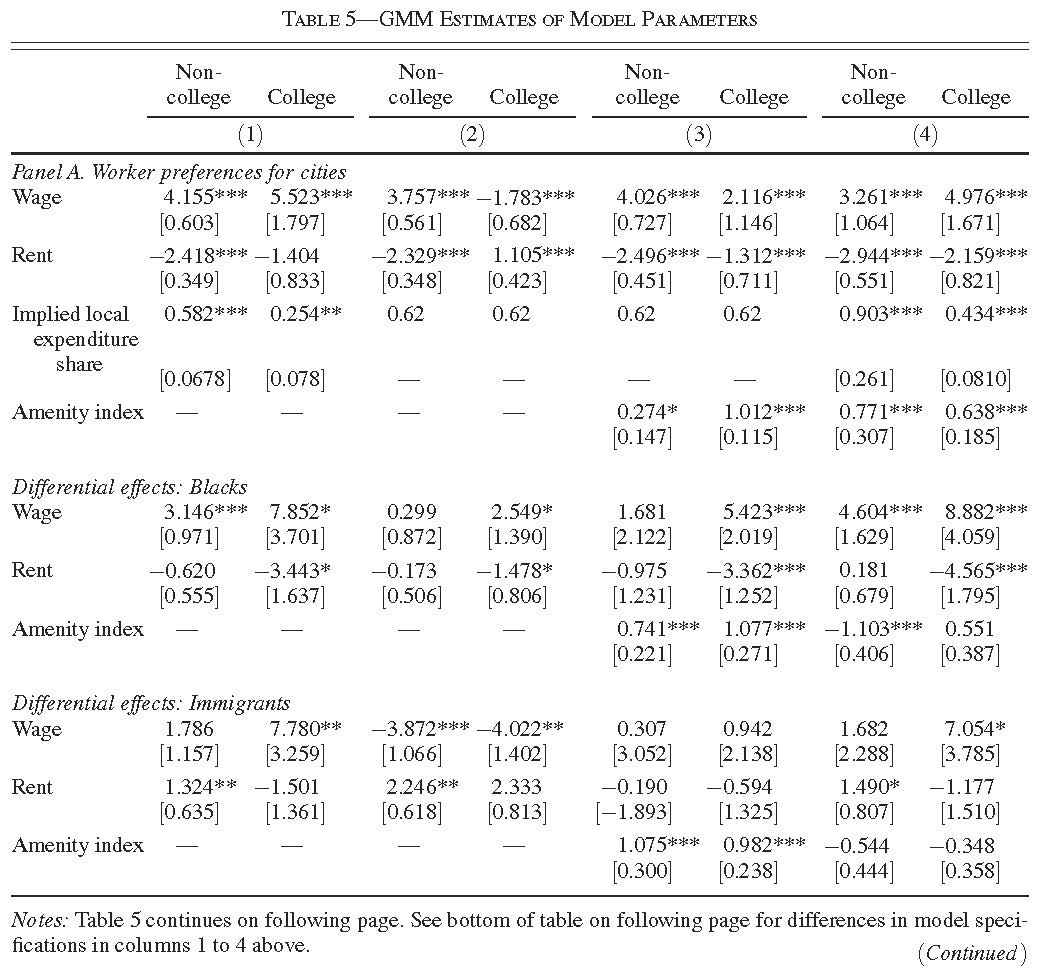
\includegraphics[scale=0.55]{DiamondTable5_1.jpg}
    \label{fig:Table5a}
\end{figure}
    
\end{frame}

%-------------------------------------------------------------

\begin{frame}{Standard and Restricted Models}

\begin{itemize}
    \item<1-> Column 1 of Table 5 shows the ``standard” model.  Both college and non-college workers prefer higher wages and lower rents. However, their willingness to trade off wages and rents are extremely different, indicating they appear to have very different expenditure shares on local goods.
    \item<2-> Consumer Expenditure Survey (CEX) from 2000 census allows us to measure local expenditure share directly, which comes out to 62\%.  2nd column of Table 5 re-runs standard model while restricting local expenditure share to 0.62.
    \item<3-> The restricted standard model seems to imply that college workers seem to \emph{prefer} lower wages and higher rents.  
\end{itemize}
    
\end{frame}

%-------------------------------------------------------------

\begin{frame}{Full Model}

\begin{itemize}
    \item<1-> The fact that college educated workers appear to be indifferent to higher local prices seems to indicate that there is an omitted variables bias, which Diamond attributes to local endogenous amenities.
    \item<2-> Column 3 of Table 5 adds the amenity index and keeps the 0.62 local expenditure restriction (she calls this the ``full” model).  This result shows that, other things equal, college workers do like higher wages and lower rents, but are somewhat less sensitive to it than non-college workers.
    \item<3-> However, college workers do have a much stronger preference for local amenities.
\end{itemize}
    
\end{frame}

%-------------------------------------------------------------

\begin{frame}{Expenditure Parameters by Demographic Groups}

\begin{itemize}
    \item<1-> Column 4 of Table 5 allows the local expenditure parameter to be estimated by group and includes the amenity index.  Expenditure shares are highly correlated with rents, so the estimate is noisier.
    \item<2-> Bottom of Panel A of Table 5 looks at differences across demographic groups.  Blacks and immigrants tend to be somewhat more sensitive to wages, rents, and amenities, but estimates are noisier.
\end{itemize}
    
\end{frame}

%-------------------------------------------------------------

\begin{frame}{Table 6}

\begin{figure}
    \centering
    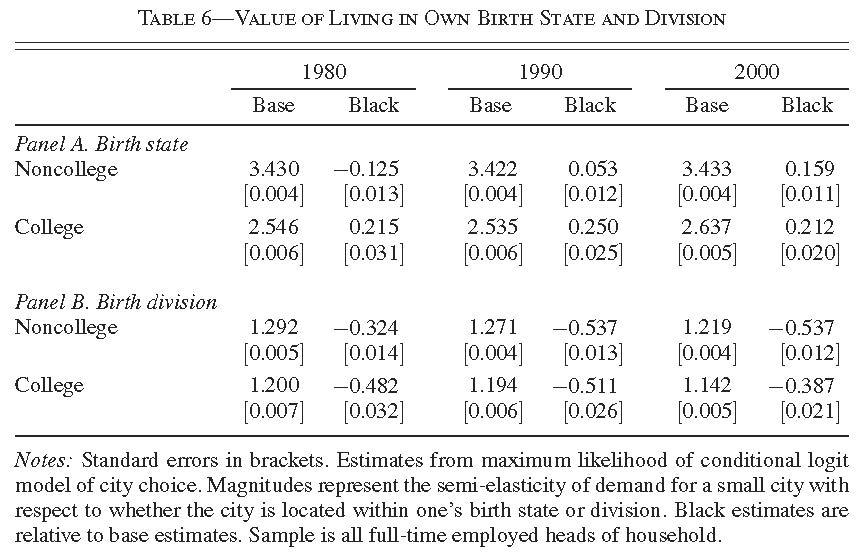
\includegraphics{DiamondTable6.jpg}
    \label{fig:Table6}
\end{figure}
    
\end{frame}

%-------------------------------------------------------------

\begin{frame}{Value of State and Census Division of Birth}

\begin{itemize}
    \item<1-> Table 6 looks at the value of living in one’s home state and census division of birth.
    \item<2->  Non-college workers are 4.4 times more likely to live in an MSA in their state of birth and college workers are only 3.5 times more likely.
    \item<3-> Same census division is 2.2 times more likely for both college and non-college workers. 
\end{itemize}
    
\end{frame}

%-------------------------------------------------------------

\subsection{Housing Supply}

%-------------------------------------------------------------

\begin{frame}{Table 5, Panels B-D}

\begin{figure}
    \centering
    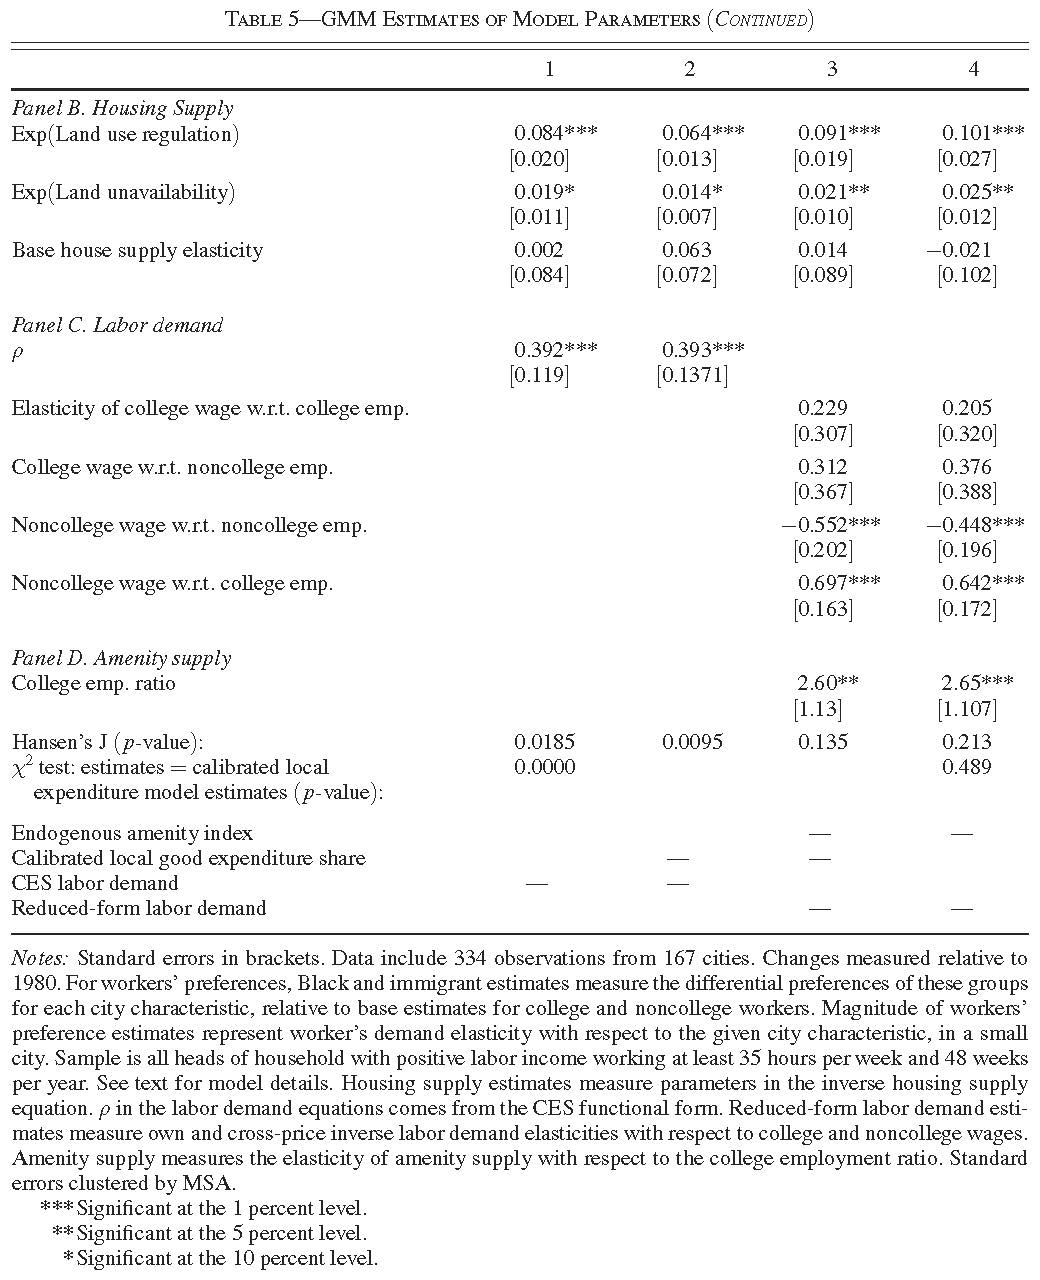
\includegraphics[scale=0.43]{DiamondTable5_2.jpg}
    \label{fig:Table5b}
\end{figure}
    
\end{frame}

%-------------------------------------------------------------

\begin{frame}{Housing Supply}

\begin{itemize}
    \item<1-> Panel B of Table 5 presents housing supply elasticity estimates.
    \item<2-> Housing supply is less elastic in MSAs with less land availability and more land use regulations.  Estimates do not vary substantially across different models.
\end{itemize}
    
\end{frame}

%-------------------------------------------------------------

\subsection{Labor Demand}

%-------------------------------------------------------------

\begin{frame}{Labor Demand}

\begin{itemize}
    \item<1-> Panel C of Table 5 shows the estimates for local labor demand curves.  Elasticity of labor substitution between college and non-college workers is almost identical at 0.392 and 0.393 in first two models.
    \item<2-> Full model allows for a more flexible labor demand curve.  Downward sloping labor demand curve is found as expected for non-college workers, and they are substitutable for college workers.
    \item<3-> Demand for college workers is more interesting.  The labor demand curve is \emph{upwards} sloping, though not significantly different than zero, but significantly greater than for non-college labor. There may be an endogenous productivity effect from having college workers around.
\end{itemize}
    
\end{frame}

%-------------------------------------------------------------

\subsection{Amenity Supply}

%-------------------------------------------------------------

\begin{frame}{Amenity Supply}

\begin{itemize}
    \item<1->  Panel D of Table 5 estimates the elasticity of the supply of the amenity index with respect to the college employment ratio.
    \item<2-> Both models report similar elasticities of amenity supply between 2.60 and 2.65.
    \item<3->  An increase in the city’s college employment ratio endogenously changes the supply of amenities in the area.
\end{itemize}
    
\end{frame}

%-------------------------------------------------------------

\subsection{Estimation Robustness}

%-------------------------------------------------------------

\begin{frame}{Estimation Robustness}

\begin{itemize}
    \item<1-> Robustness checks with several different variable definitions are in an Appendix.
    \item<2-> Details are online, but no very interesting results.
\end{itemize}
    
\end{frame}

%-------------------------------------------------------------

\section{Amenities and Productivity Across Cities}

%-------------------------------------------------------------

\begin{frame}{Amenities and Productivity Across Cities}

\begin{itemize}
    \item<1->  With estimated parameters, one can infer the exogenous productivity of local firms and desirability of local amenities in each city.
    \item<2-> Going by the indirect utility function (\ref{eq:deltaamenities2}), we can derive the utility that workers of type $ z $ receive from amenities in city $ j $ in year $ t $ as:
    \begin{equation*}
        Amen_{j,t}^{z} = \beta_{i}^{a} a_{j,t} + \zeta_{j,t}^{z} = \beta^{w} z\left( w_{j,t}^{edu} - \xi r_{j,t} \right)
    \end{equation*}
    \item<3->  Basic idea is that amenities are inferred to be the highest in cities which have higher population levels of a given demographic group than expected given the city’s wage and rent levels.
\end{itemize}
    
\end{frame}

%-------------------------------------------------------------

\begin{frame}{Amenities and Productitivity Across Cities}

\begin{itemize}
    \item<1-> Results seem to conform with intuition.  Large coastal cities have the highest estimated amenity indexes, whereas the lowest estimated amenity indexes tend to be in rust-belt cities.  Some differences exist between college and non-college workers, but they are not very different.
    \item<2-> Biggest increases in productivity for high-skill workers were in major tech hubs.
    \item<3-> Biggest increases in productivity for low-skill workers were in metro areas that had lots of agricultural production and/or shipping centers with jobs that are difficult to offshore.
\end{itemize}
    
\end{frame}

%-------------------------------------------------------------

\begin{frame}{Table 7}

\begin{figure}
    \centering
    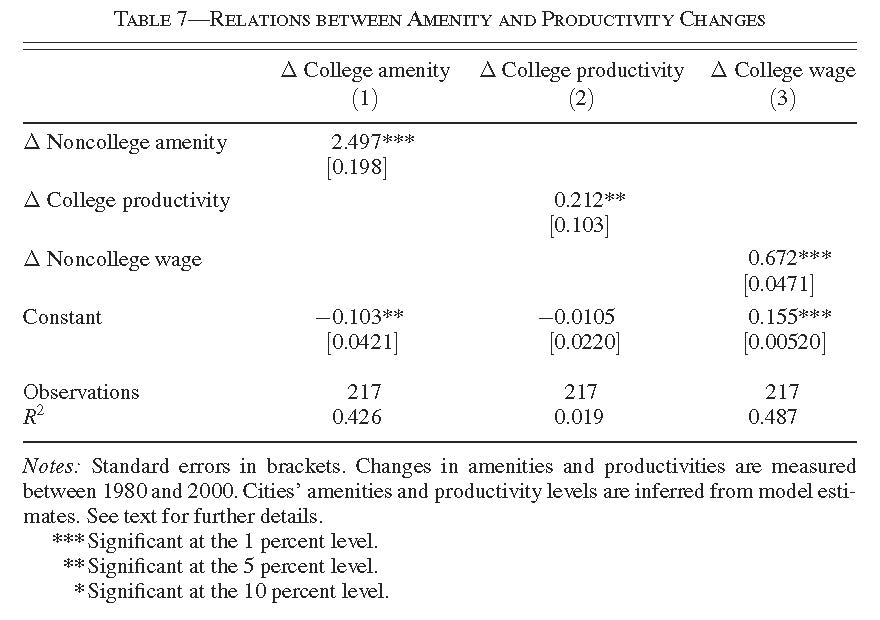
\includegraphics[scale=0.85]{DiamondTable7.jpg}
    \label{fig:Table7}
\end{figure}
    
\end{frame}

%-------------------------------------------------------------

\begin{frame}{Relationship Between Amenities and Productivity Changes}

\begin{itemize}
    \item<1-> Table 7 shows the relationship between amenities changes and productivity changes.
    \item<2-> Amenity changes are strongly correlated with each other.
    \item<3-> College and non-college productivities are weakly correlated with each other.
    \item<4-> College and non-college wages are strongly correlated with each other.
\end{itemize}
    
\end{frame}

%-------------------------------------------------------------

\section{The Determinants of Cities’ College Employment Ratio Changes}

\subsubsection{College Employment Ratio Changes and Productivity}

%-------------------------------------------------------------

\begin{frame}{College Employment Ratio Changes and Productivity}

\begin{itemize}
    \item<1-> Changes in local productivity directly impact wages, but also influence local prices and amenities through migration.
    \item<2-> The direct effect of exogenous productivity changes from 1980 to 2000 are inferred from the model and high and low skill wages:
    \begin{equation*}
        \begin{split}
            \hat{w}_{j,2000}^{H} &= \gamma_{HH} \log\left( H_{j,1980} \right) + \gamma_{HL} \log\left( L_{j,1980} \right) + \varepsilon_{j,2000}^{H} \\
            \hat{w}_{j,2000}^{L} &= \gamma_{LH} \log\left( H_{j,1980} \right) + \gamma_{LL} \log\left( L_{j,1980} \right) + \varepsilon_{j,2000}^{L}
        \end{split}
    \end{equation*}
    where  $ \hat{w}_{j,2000}^{H} $ and $ \hat{w}_{j,2000}^{L} $ are the counter factual high and low skill wages driven by exogenous productivity shocks and initial labor market composition.
\end{itemize}
    
\end{frame}

%-------------------------------------------------------------

\begin{frame}{College Employment Ratio Changes and Productivity}

Using the counter factual wages and the amenity levels of 1980, we can use the model to predict where workers would live in a set of hypothetical cities with 2000 wages and 1980 amenities:
\begin{equation*}
    V_{i,j,t} = \left( \hat{w}_{j,2000}^{edu} - \xi r_{j,1980} \right) \beta^{w} z_{i} + a_{j,1980} \beta_{i}^{a} + x_{j,1980} \beta_{i}^{x} + x_{j}^{st}\beta_{i}^{st} + x_{j}^{div} \beta_{i}^{div} + \varepsilon_{i,j,1980}
\end{equation*}
Predicted cities’ college employment ratios from this hypothetical world are compared to those observed in the data. 
    
\end{frame}

%-------------------------------------------------------------

\begin{frame}{Figure 2}

\begin{figure}
    \centering
    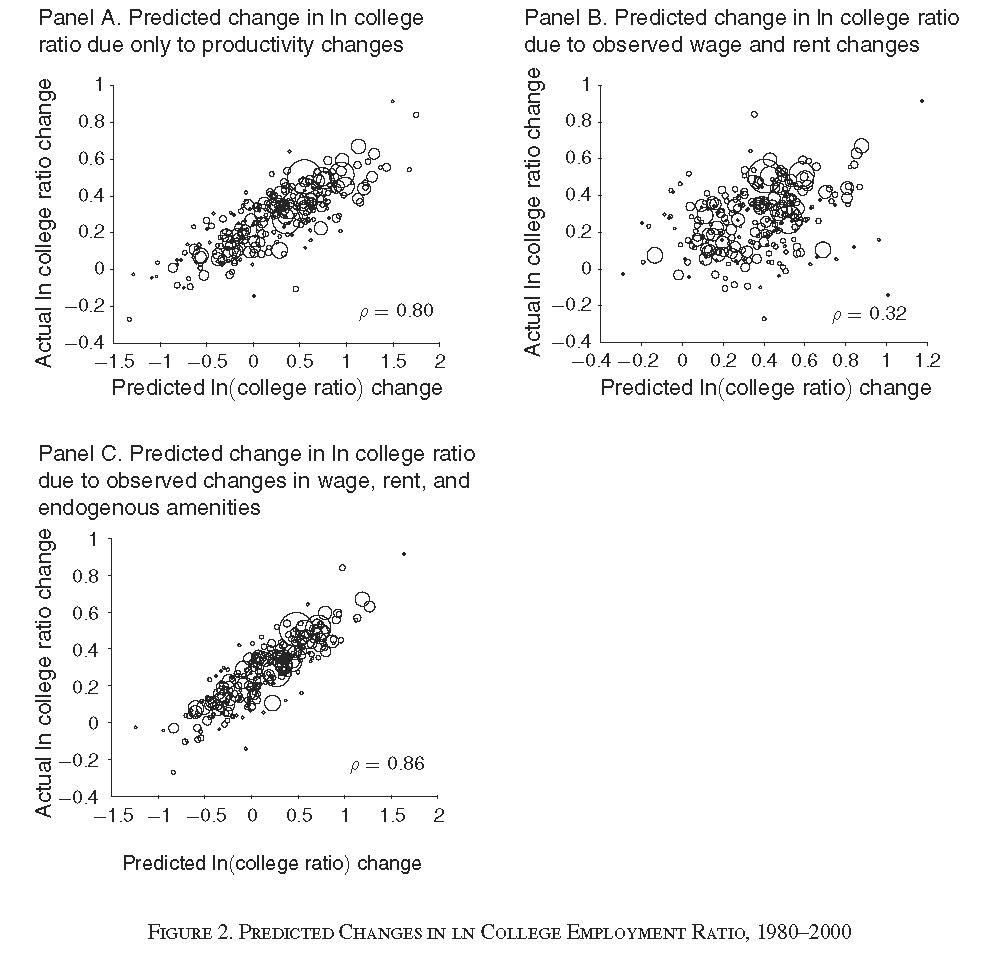
\includegraphics[scale=0.57]{DiamondFig2.jpg}
    \label{fig:Figure2}
\end{figure}
    
\end{frame}

%-------------------------------------------------------------

\begin{frame}{Counter Factuals vs. Observed Employment Ratios}

\begin{itemize}
    \item<1-> Panel A of Figure 2 shows the correlation of the observed college employment ratios against the counter factual ratios.  The correlation between these is strongly positive with a coefficient of 0.80.
    \item<2-> If endogenous amenity changes were not an important factor in how productivity changes influenced cities’ college employment ratio changes, then local wage and rent changes should be at least as strong of a predictor of college employment ratio changes.
    \item<3-> Panel B plots observed college employment ratio changes against predicted college employment ratio changes.  The correlation is positive, but only 0.32, which suggests that amenity changes are important component through which cities’ college employment ratios change.
    \item<4-> Panel C repeats this analysis, but plots actual college employment ratio changes against changes predicted due to wages, rents, and endogenous amenities.  The correlation coefficient is now 0.86, indicating that the combination of these three factors is important.
\end{itemize}
    
\end{frame}

%-------------------------------------------------------------

\section{Welfare Implications for Well-Being Inequality}

%-------------------------------------------------------------

\begin{frame}{Welfare Implications for Well-Being Inequality}

\begin{itemize}
    \item<1-> Initial analysis showed that the nationwide college wage gap increased by 19\% between 1980 and 2000.  But there may be a greater change due to residence choices.
    \item<2->  Local real wage gap, which takes into account rents, has increased by 15\%.  But this doesn’t capture why college graduates pay higher rents.
    \item<3-> To measure how changes in cities wages, rents, and amenities each contribute to well-being inequality, the paper conducts a welfare decomposition.
\end{itemize}
    
\end{frame}

%-------------------------------------------------------------

\begin{frame}{Table 9}

\begin{figure}
    \centering
    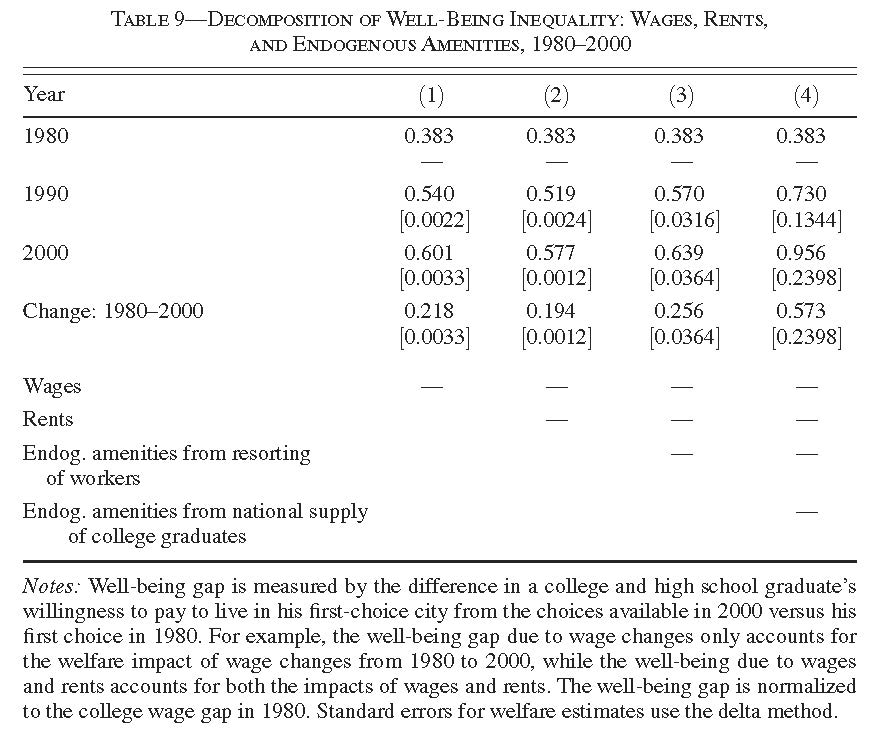
\includegraphics[scale=0.7]{DiamondTable9.jpg}
    \label{fig:Table9}
\end{figure}
    
\end{frame}

%-------------------------------------------------------------

\begin{frame}{Well-Being Inequality}

\begin{itemize}
    \item<1->  First step, measure each worker’s expected utility change from 1980 to 2000 if only wages had changed, but local rents and amenities stayed constant.  Table 9 shows these results.  Utility gap due to wages only is equal to 21.8\%.
    \item<2-> Column 2, which accounts for local rent changes, has a gap of 19.4\%.
    \item<3-> Column 3 looks at impact of amenity changes holding the national share of college labor constant and only looking at re-sorting of workers across MSAs.  Gap increases to 25.6\%.
    \item<4->  Finally, Column 4 allows the national share of college labor to change and have average level of amenities adjust to increase in college labor.  Gap widens significantly to 57.3\%.
\end{itemize}
    
\end{frame}

%-------------------------------------------------------------

\section{Conclusions}

%-------------------------------------------------------------

\begin{frame}{Conclusions}

\begin{itemize}
    \item<1->  Between 1980-2000, there was an increase in the wage gap in the U.S. between college-educated and non-college-educated labor as well as an increase in the share of college-educated labor.
    \item<2->  At the same time, college educated workers began to disproportionately concentrate in nicer but more expensive cities.
    \item<3->  Diamond shows that this labor sorting raised the welfare of college-educated workers over and above what is accounted for by looking at nominal wages.
\end{itemize}
    
\end{frame}

%-------------------------------------------------------------

\begin{frame}{Conclusions}

\begin{itemize}
    \item<1->  Why do we care?  International trade is blamed in part for the increase in wage dispersion.
    \item<2->  If new and better jobs are being created in some parts of the country, and not in others, it may be harder for people to adjust to the shocks from trade.
\end{itemize}
    
\end{frame}

%-------------------------------------------------------------

\end{document}